\hfill\break
\justifying
Como penúltima sección se tienen a las operaciones morfológicas. Del área de estudio Morfología Matemática desarrollada por los hermanos Minkosky, la idea básica detrás de la Morfología Matemática es probar una imagen pormedio de un probador, que se denomina Elemento de Estructura(EE), y cualificar de esta manera en que dicho EE encaja, o no, una imagen.

\hfill\break
\justifying
Ayudándose del marcado de los EE que si encajan en un objeto, uno es capaz de derivar información relacionada con la estructura relativa a la imagen y el objeto.

\hfill\break
\justifying
La información que se obtenga dependerá del tamaño del EE así como de su forma, siendo de gran importancia la elección de un EE correcto.

\hfill\break
\justifying
Dos operaciones dentro de la teoría de la Matemática Morfológica son escenciales, y es que son la base de la derivación de las demás operaciones:

\subsection*{Operaciones básicas}
	\subsubsection*{Erosión}
		\hfill\break
		\justifying
		\textbf{Formalmente}: Sean \textit{A} y \textit{B} 2 conjuntos en $Z^2$, la erosión de \textit{A} por \textit{B} denotada como $A\Theta B$ se define como:
		\begin{equation*}
			A\Theta B = {x|(B)_x\subseteq A}
		\end{equation*}
	
		\hfill\break
		\justifying
		En otras palabras, la erosión de \textit{A} por \textit{B} es el conjunto de todos los puntos \textit{x} tal que \textbf{B} trasladada por \textit{x} está contenida en \textit{A}.
		
		\hfill\break
		\justifying
		Visualmente el resultado que se obtiene de aplicar una erosión es el adelgazamiento de la figura en la que se aplica, esto por supuesto, influenciado por la forma de la estructura EE.
		
	\subsubsection*{Dilatación}
		\hfill\break
		\justifying
		\textbf{Formalmente:} Sean \textit{A} y \textit{B} 2 conjuntos en $Z^2$, la dilatación de \textit{A} por \textit{B}, denotada como $A\oplus B$ se define como:
		\begin{equation*}
			A\oplus B = {x|\hat{B_x} \cap A \neq \oslash}
		\end{equation*}
	
		\hfill\break
		\justifying
		En otras palabras, el proceso de dilatación consiste en obtener la reflexión del elemento estrsucturante \textit{B} al rededor de su origen y después desplazar esta reflexión por \textit{x}. $A\oplus B$ es entonces el conjunto de todos los desplazamientos en \textit{x} tales que $\hat{B}$ y \textit{A} comparten al menos un elemento no igual al cero.
		
		\hfill\break
		\justifying
		Visualmente después de aplicar la dilatación sobre un objeto este se notará más ensanchado. La capacidad de que el objeto conserve su forma original dependerá de la elección del EE y su tamaño.

\subsubsection*{Operaciones derivadas}
	\hfill\break
	\justifying
	Con el objeto de aumentar el efecto de las operaciones básicas, se pueden diseñar filtros consistentes ne la iteración de varias operaciones de erosión o de dilatación.
	
	\hfill\break
	\justifying
	En ocasiones la aplicación de 1 sola iteración de operaciones no da el resultado esperado, por lo que es necesario el encadenamiento de n iteraciones de filtrado para obtener el resultado.
	
	\hfill\break
	\justifying
	El uso de las operaciones básicas en conjunto es común en este tipo de iteraciones, y sin embargo es fácil pensar que las operaciones de dilatación y erosión son opuesta, pero es en general no es cierto, de forma que implementación conjunta da apertura a nuevas operaciones.
	
	\subsubsection*{Apertura Morfológica}
		\hfill\break
		\justifying
		\textbf{Formalmente:} Sean \textit{A} y \textit{B} dos conjuntos en $Z^2$, la apertura de \textit{A} por \textit{B}, denotada como $A \circ B$ se define como:
		\begin{equation*}
			A \circ B = (A\Theta B) \oplus B
		\end{equation*}
	
		\hfill\break
		\justifying
		En otras palabras, la apertura de \textit{A} por \textit{B} es simplemente y sencillamente la erosión de \textit{A} por \textit{B} seguida de la dilatación del resultado.
		
	\subsubsection*{Cerradura Morfológica}
		\hfill\break
		\justifying
		\textbf{Formalmente:} Sean \textit{A} y \textbf{B} dos conjuntos en $Z^2$, la cerradura de \textit{A} por \textit{B}, denotada como $A \bullet B$, se define como:
		\begin{equation*}
			A\bullet B = (A\oplus B)\Theta B
		\end{equation*}
	
		\hfill\break
		\justifying
		En otras palabras, la cerradura de \textit{A} por \textbf{B} es simple y sencillamente la dilatación de \textit{A} por \textbf{B} seguida de la erosión del resultado.

\subsubsection{Implementación}
	\hfill\break
	\justifying
	A continuación se ejemplifica el poder de las operaciones morfológicas en una situación donde se cuenta con una imagen de monedas que pueden ser contadas con el algoritmo básico de \textbf{bit-quad}, sin embargo la sola binarización con un umbral no da un resultado para implementarlo, de forma que aplicando en cadena las operaciones se consigue limpiar perfectamente la imagen binarizada para aplicar en el algoritmo de contabilización de objetos.
	
	\begin{figure}[!h]
		\centering
		\begin{tabular}{cc}
			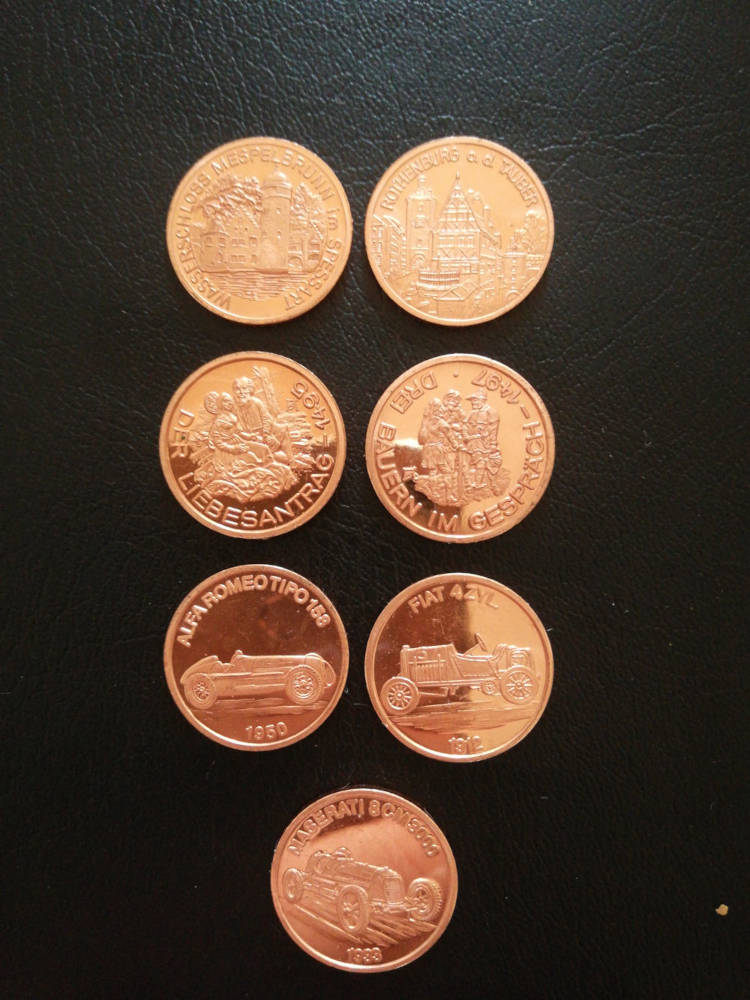
\includegraphics[width=7.5cm]{Imagenes/monedas_2_chica.jpeg} & 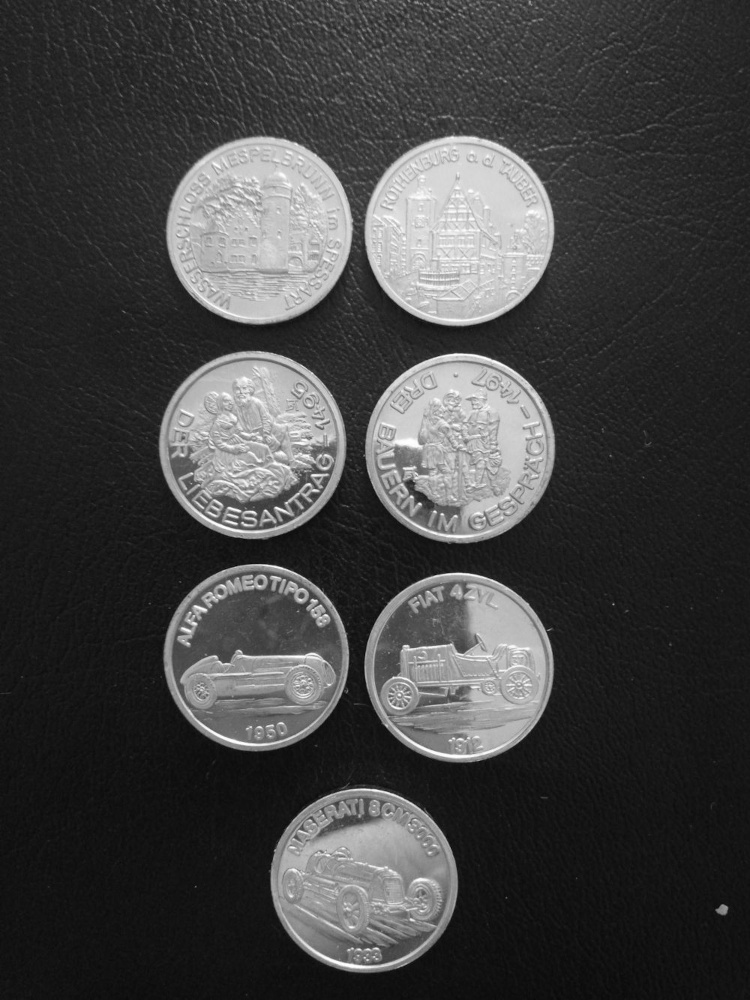
\includegraphics[width=7.5cm]{Imagenes/op_morf_monedas_0.jpeg}
		\end{tabular}
		\caption{1) Imagen original de las monedas. Colocadas sobre un fondo obscuro con gran contraste, nos enfrentamos a la textura tipo vinil que con la iluminación no es completamente negro \\ 2) Transformación a escala de grises de la imagen original}
	\end{figure}

	\newpage

	\begin{figure}[!h]
		\centering
		\begin{tabular}{cc}
			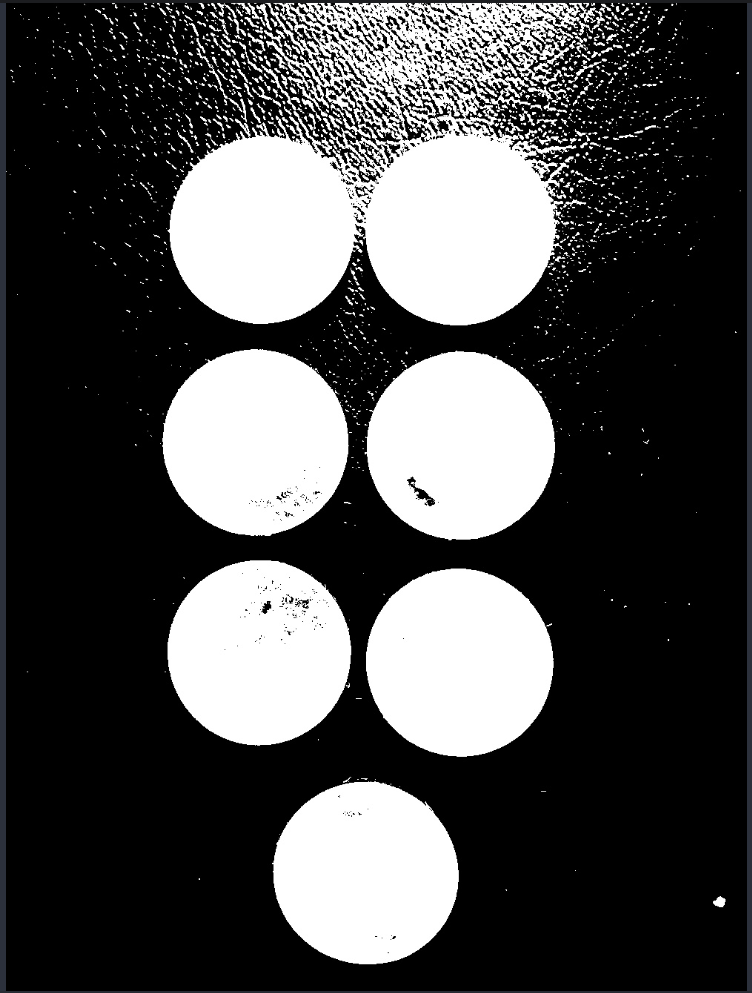
\includegraphics[width=7.5cm]{Imagenes/op_morf_monedas_1.png} & 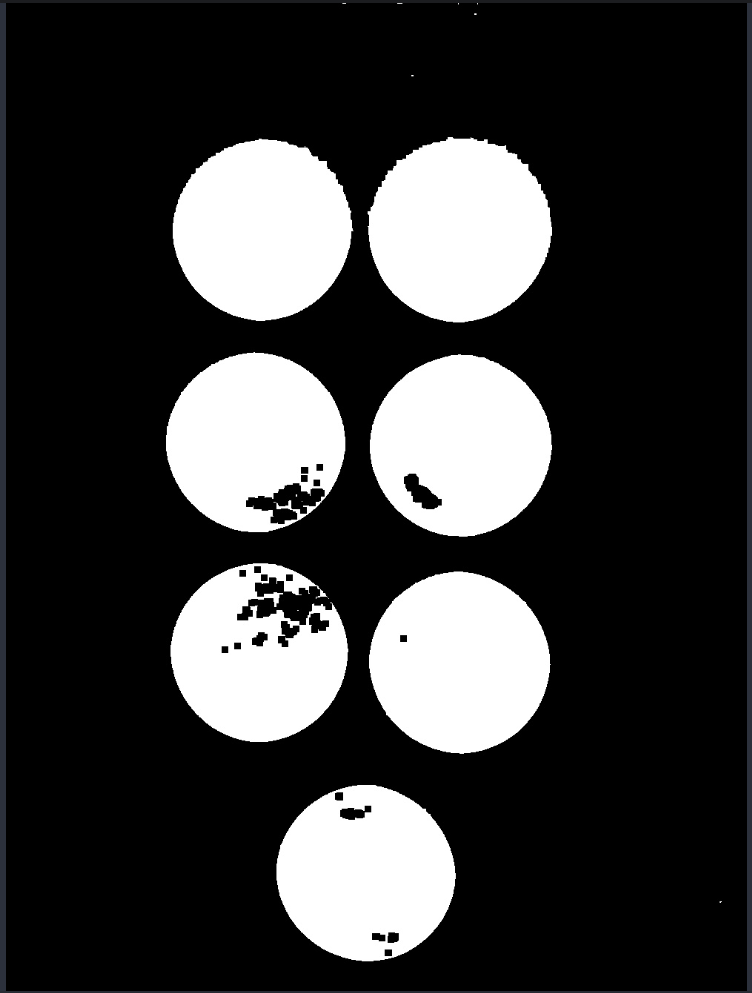
\includegraphics[width=7.5cm]{Imagenes/op_morf_monedas_2.png} \\
			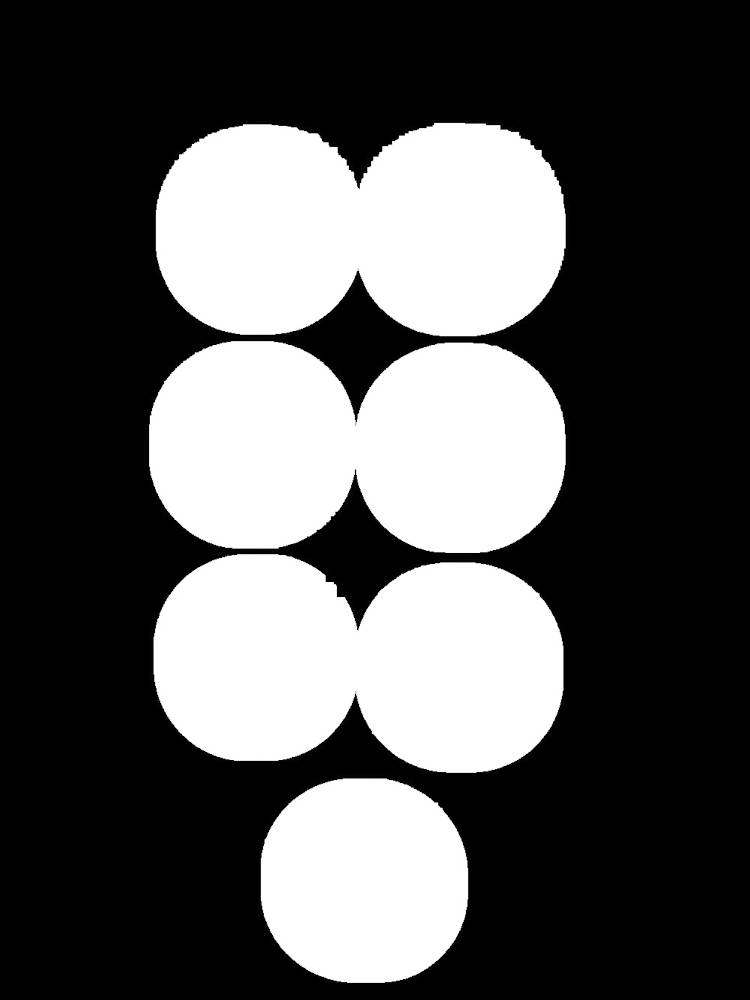
\includegraphics[width=7.5cm]{Imagenes/op_morf_monedas_3.jpeg} & 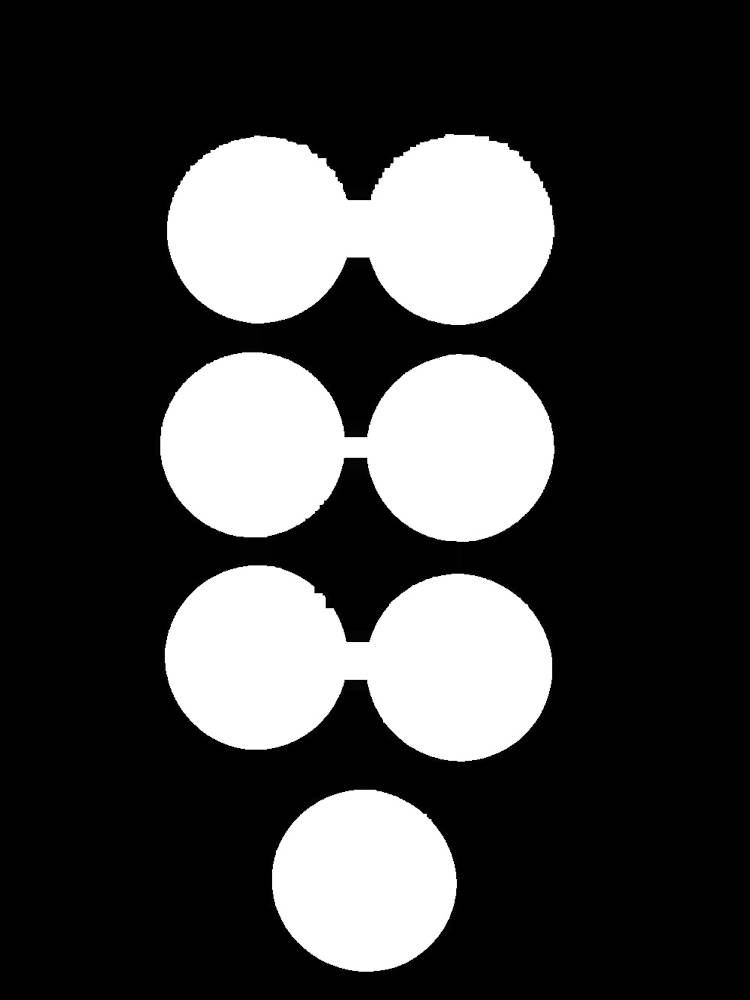
\includegraphics[width=7.5cm]{Imagenes/op_morf_monedas_4.jpeg} 
		\end{tabular}
		\caption{1) Binarización de la imagen con un umbral manual de 60. Se aprecia que debido a la textura en la parte superior la binarización no lo colorea como el fondo\\ 2) Aplicando una operación de erosión con un kernel grande de $n=9$ se elimina casi por completo las textura mal coloreada. Se termina por aplicar una erosión más con un kernel pequeño de $n=3$. \\ 3) Para poder rellenar los espacios en negro dentro las monedas se aplican consecutivamente 3 dilataciones con kernel $n=9$ y 1 dilatación con $n=5$. Se han rellenado las monedas pero se encuentran unidas. \\ 4) Aplicando consecutivamente la erosión con kernel grande de $n=12$ se separan las monedas. }
	\end{figure}

	\newpage

	\begin{figure}[!h]
		\centering
		\begin{tabular}{cc}
			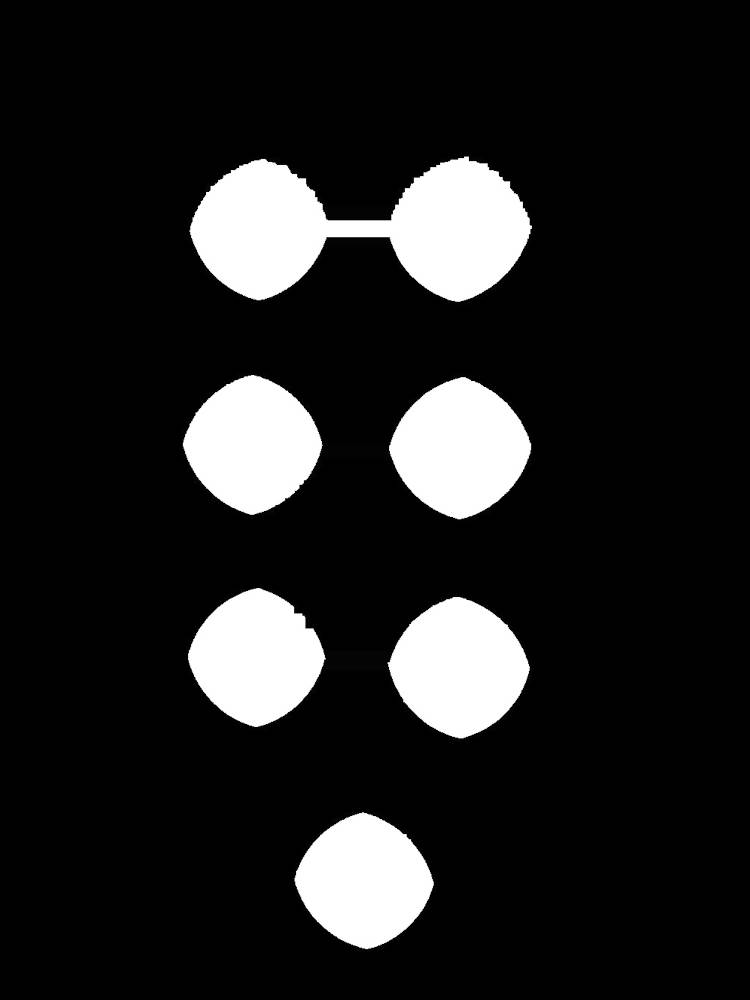
\includegraphics[width=7.5cm]{Imagenes/op_morf_monedas_5.jpeg} & 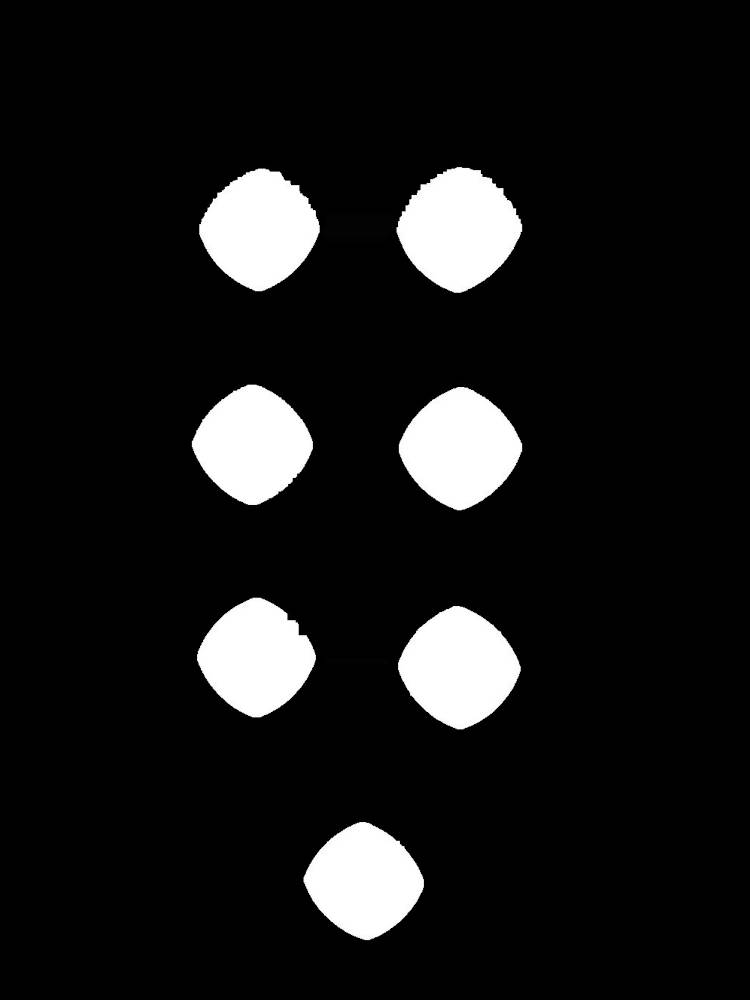
\includegraphics[width=7.5cm]{Imagenes/op_morf_monedas_6.jpeg} \\
			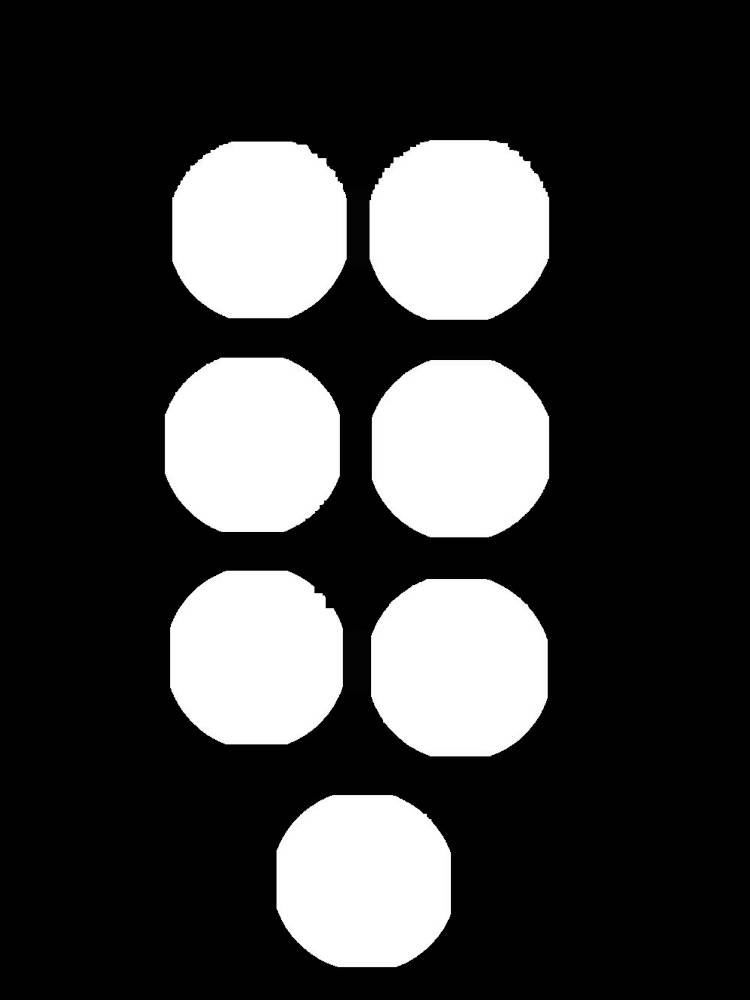
\includegraphics[width=7.5cm]{Imagenes/op_morf_monedas_final.jpeg} &
			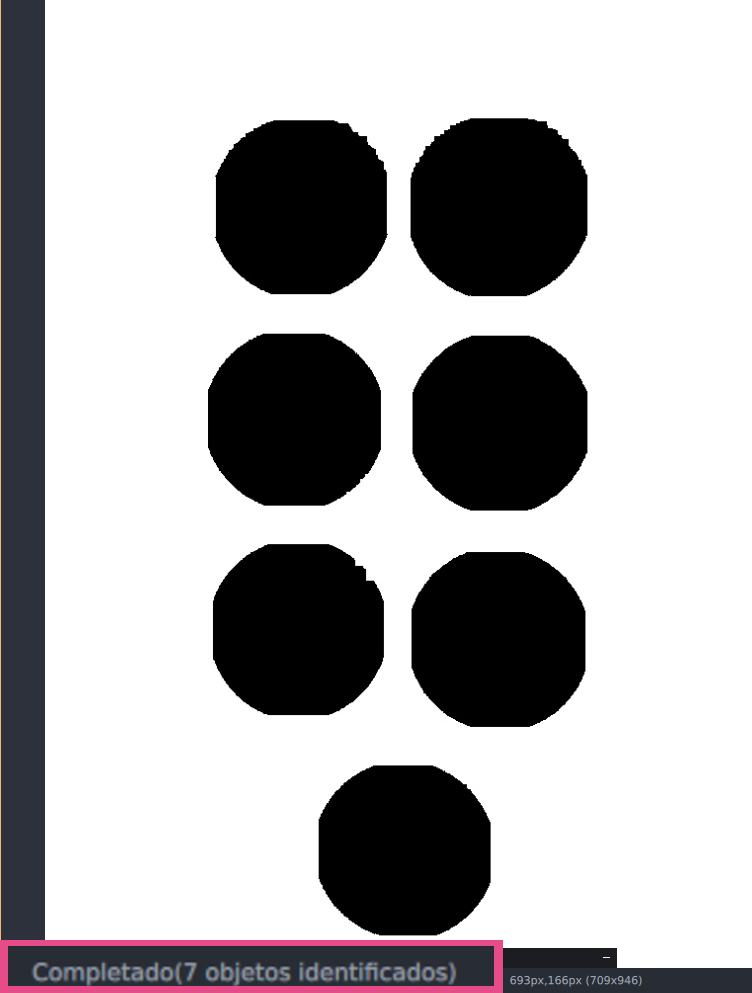
\includegraphics[width=7.5cm]{Imagenes/op_morf_monedas_contabilizacion.png}
		\end{tabular}
		\caption{1) Se encuentran casi en su totalidad separadas las monedas, resta eliminar esa unión utilizando la apertura con un kernel $n=9$. \\ 2) Se han rellenado y recuperado las monedas que había en un principio, sin embargo el tamaño aún no es el correcto por lo que deben aplicarse 7 dilataciones con kernel $n=12$.\\ 3) Una vez recuperada la forma y el tamaño casi original de las monedas se puede procesar y tratar la imagen como más se requiera, en este caso realizando la contabilización de los objetos. \\ 4) Importante señalar que típicamente los objetos se colorean de color negro y el fondo de color claro, por lo que la inversión de colores es requerida antes de invocar la contabilización.}
	\end{figure}
	
	\newpage
	
	\hfill\break
	\justifying
	La implementación de las operaciones morfológicas es bastante sencilla cuando se aprovechan las herramienta de la biblioteca OpenCV, existiendo ya como función las operaciones Erosión y Dilatación, a las cuales basta pasarles como argumento el elemento de estructura con su tamaño y forma especificada. Para la apertura y cerradura se cuenta con una función más general que recibe el tipo de operación a realizar identificado por una constante de la misma biblioteca y el elemento estructural como tercer argumento.

	\begin{lstlisting}[language=Python]
		def morphological_operation(morph_op_type:str,image,n:int=3,spatial_structure:str='rect',**kargs):
			image = copy(image)
			structuring_element = cv2.getStructuringElement(cv2.MORPH_CROSS if spatial_structure == 'cross' else cv2.MORPH_RECT,(n,n))
			
			if morph_op_type == 'erosion':
			return cv2.erode(image,structuring_element)
			elif morph_op_type == 'dilation':
			return cv2.dilate(image,structuring_element)
			elif morph_op_type == 'closing':
			return cv2.morphologyEx(image,cv2.MORPH_CLOSE,structuring_element)
			elif morph_op_type == 'opening':
			return cv2.morphologyEx(image,cv2.MORPH_OPEN,structuring_element)
	\end{lstlisting}
